In questa sezione verranno elencati ed analizzati tutti i casi d'uso$^*$ individuati dal gruppo. Ogni caso d'uso verrà identificato da un codice univoco secondo le regole descritte nel documento \textit{Norme di progetto} e riportate di seguito. 

\subsection{Denominazione dei casi d'uso}
Ad ogni caso d'uso saranno associate le seguenti informazioni:
\begin{itemize}
\item il codice del requisito che lo interessa UC-[Codice];
\item un nome (univoco);
\item le pre-condizioni e le post-condizioni relative allo specifico caso d'uso;
\item gli attori coinvolti, sia primari che secondari;
\item lo scenario principale che il caso d'uso vorrebbe modellare;
\item le eventuali estensioni dello scenario principale.
\end{itemize}

\subsubsection{Gerarchie dei casi d'uso} 
Gli identificatori numerici assegnati a casi d'uso saranno organizzati gerarchicamente. Posto UC-X codice di un caso d'uso, allora UC-X.Y è figlio di UC-X ed esiste fra i due una relazione tra quelle elencate:
\begin{itemize}
\item UC-X.Y descrive nel dettaglio una delle funzionalità di UC-X;
\item UC-X.Y descrive una estensione (o scenario alternativo) dello scenario descritto in UC-X; 
\item UC-X.Y descrive una estensione dello scenario principale di due o più figli di UC-X.
\end{itemize}

\subsection{Elenco dei casi d'uso - Utente generico}

	\subsubsection{UC-39 Inserimento di una frase da svolgere}
	\begin{itemize}
		\item \textbf{Attori:} Utente generico.
		\item \textbf{Precondizione:} L'utente visualizza la vista principale dell'applicazione.
		\item \textbf{Postcondizione:} L'utente visualizza la vista per l'esecuzione dell'esercizio.
		\item \textbf{Scenario principale:}
		\begin{enumerate}
			\item l'utente scrive la frase da svolgere come esercizio
			\item l'utente conferma la frase indicata
		\end{enumerate}
	\end{itemize}

	\subsubsection{UC-40 Selezione esercizio da svolgere}
	\begin{itemize}
			\item \textbf{Attori:} Utente generico.
			\item \textbf{Precondizione:} L'utente visualizza la lista degli esercizi ricercati.
			\item \textbf{Postcondizione:} L'utente visualizza la vista per l'esecuzione dell'esercizio.
			\item \textbf{Scenario principale:}
			\begin{enumerate}
					\item l'utente seleziona l'esercizio da svolgere
			\end{enumerate}
	\end{itemize}

	\subsubsection{UC-6 Ricerca esercizi}
		\begin{itemize}
			\item\textbf{ Attori:} Utente generico
			\item \textbf{Precondizione:} L'utente si trova nella vista principale dell'applicazione.
			\item \textbf{Postcondizione:} L'utente ottiene una lista degli esercizi filtrati.
			\item \textbf{Scenario principale:}
				\begin{enumerate}
					\item l'utente accede all'area dedicata alla ricerca degli esercizi
					\item l'utente scrive la frase o una sua parte nella barra di ricerca
					\item l'utente seleziona i filtri (UC-6.1)
					\item l'utente avvia la ricerca
				\end{enumerate}
		\end{itemize}

	\subsubsection{UC-6.1 Filtraggio esercizi }
		\begin{itemize}
			\item \textbf{Attori:} Utente generico.
			\item \textbf{Precondizione:} L'utente si trova nella vista di ricerca degli esercizi dell'applicazione.
			\item \textbf{Postcondizione:} L'utente ha selezionato i filtri per la ricerca.
			\item \textbf{Scenario principale:}
				\begin{enumerate}
					\item l'utente può selezionare gli autori degli esercizi desiderati (UC-6.1.1)
					\item l'utente può selezionare il livello di difficoltà degli esercizi (UC-6.1.2)
					\item l'utente può selezionare gli argomenti degli esercizi (UC-6.1.3)
				\end{enumerate}
		\end{itemize}
		
		\begin{figure}[h]
			\centering
			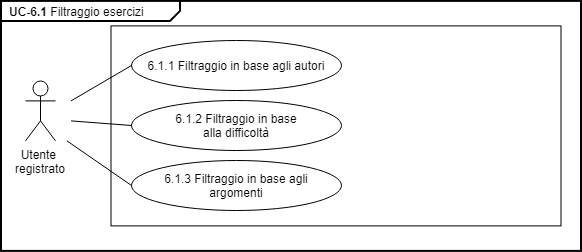
\includegraphics[scale=0.7]{images/UC-6.png}
			\caption{UC-6 Filtraggio esercizi}
		\end{figure}	

\subsubsection{UC-6.1.1 Filtraggio in base agli autori}
	\begin{itemize}
		\item \textbf{Attori:} Utente generico
		\item \textbf{Precondizione: } L'utente si trova nella vista di ricerca degli esercizi dell'applicazione.
		\item \textbf{Postcondizione: } L'utente ha indicato gli autori nel filtro di ricerca.
		\item \textbf{Scenario principale:}
		\begin{enumerate}
			\item l'utente visualizza la lista degli autori
			\item l'utente seleziona gli autori di cui vuole vedere gli esercizi
		\end{enumerate}
	\end{itemize}

\subsubsection{UC-6.1.2 Filtraggio in base alla difficoltà}
	\begin{itemize}
		\item \textbf{Attori:} Utente generico
		\item \textbf{Precondizione: } L'utente si trova nella vista di ricerca degli esercizi dell'applicazione.
		\item \textbf{Postcondizione: } L'utente ha indicato la difficoltà nel filtro di ricerca.
		\item \textbf{Scenario principale:}
		\begin{enumerate}
			\item l'utente visualizza i livelli possibili di difficoltà (da 1 a 5)
			\item l'utente indica il livello di difficoltà degli esercizi cercati
		\end{enumerate}
	\end{itemize}

	\subsubsection{UC-6.1.3 Filtraggio in base agli argomenti}
		\begin{itemize}
			\item \textbf{Attori:} Utente generico
			\item \textbf{Precondizione: } L'utente si trova nella vista di ricerca degli esercizi dell'applicazione.
			\item \textbf{Postcondizione: } L'utente ha indicato gli autori nel filtro di ricerca.
			\item \textbf{Scenario principale:}
			\begin{enumerate}
				\item l'utente visualizza la lista degli argomenti (pronomi, verbi, aggettivi, articoli, avverbi, ecc..)
				\item l'utente seleziona gli argomenti di cui vuole vedere gli esercizi
			\end{enumerate}
		\end{itemize}

	\subsubsection{UC-13 Svolgimento esercizio}
		\begin{itemize}
			\item \textbf{Attori:} Utente generico.
			\item \textbf{Precondizione:}  L'utente visualizza la vista per l'esecuzione dell'esercizio.
			\item \textbf{Postcondizione:} L'utente visualizza la valutazione dell'esercizio.
			\item \textbf{Scenario principale:}
				\begin{enumerate}
					\item l'utente compila i campi (UC-13.1).
					\item l'utente conferma i dati inseriti.
					\item l'utente visualizza la valutazione (UC-13.2).
				\end{enumerate}
		\end{itemize}
			
		\begin{figure}[h]
			\centering
			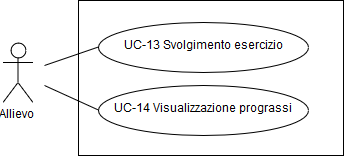
\includegraphics[scale=0.7]{images/UC-13.png}
			\caption{UC-13 Svolgimento esercizio}
		\end{figure}

	\subsubsection{UC-13.1 Compilazione dei campi}
		\begin{itemize}
			\item \textbf{Attori:} Utente generico.
			\item \textbf{Precondizione:} L'utente ha selezionato un esercizio da eseguire.
			\item \textbf{Postcondizione:} L'utente ha compilato i campi proposti dall'esercizio.
			\item \textbf{Scenario principale:}
				\begin{enumerate}
					\item l'utente sceglie la classe grammaticale per ogni parola presentata
					\item l'utente conferma la soluzione dell'esercizio
				\end{enumerate}
		\end{itemize}

	\subsubsection{UC-13.2 Visualizzazione della valutazione dell'esercizio}
	\begin{itemize}
			\item \textbf{Attori:} Utente generico.
			\item \textbf{Precondizione:} L'utente ha completato l'esecuzione dell'esercizio.
			\item \textbf{Postcondizione:} L'allievo visualizza la valutazione dell'esercizio.
			\item \textbf{Scenario principale:}
				\begin{enumerate}
					\item l'allievo seleziona il correttore dell'esercizio (insegnante o algoritmo automatico)
					\item l'allievo visualizza la valutazione (da 1 a 10) in base al correttore scelto
				\end{enumerate}
	\end{itemize}				

\subsubsection{UC-46 Segnalazione abuso di un esercizio}
	\begin{itemize}
		\item \textbf{Attori:} Utente generico
		\item \textbf{Precondizione:} L'utente si trova nella vista di svolgimento di un esercizio che ritiene non conforme alle norme di comportamento.
		\item \textbf{Postcondizione:} L'utente ha inviato una notifica di abuso del codice di comportamento.
		\item \textbf{Scenario principale:}
		\begin{enumerate}
			\item l'utente seleziona l'opzione "Segnala abuso"
		\end{enumerate}
	\end{itemize}

\subsection{Elenco dei casi d'uso - Utente: utente non registrato}

\subsubsection{UC-1 Registrazione Allievo}
\begin{itemize}
		\item \textbf{Attori: }Utente non registrato.
		\item \textbf{Precondizione: }L'utente si trova nella vista di registrazione dell'applicazione.
		\item \textbf{Postcondizione: }L'utente è registrato come allievo.
		\item \textbf{Scenario principale: }
		\begin{enumerate}
		\item l'utente ha scelto di registrarsi al sistema, quindi di creare un nuovo profilo
		\item l'utente seleziona la tipologia allievo
		\item l'utente inserirà nome, cognome, username, email e password
		\item l'utente fornirà il nome della scuola a cui appartiene e la città
		\item l'utente conferma la registrazione
		\end{enumerate}
		\item \textbf{Estensioni: }
		\begin{itemize}
			\item 5.a Nel caso in cui l'utente tenti l'inserimento di campi non validi vedrà comparire un messaggio d'errore "Campi non validi" (UC-5).
		\end{itemize}
\end{itemize}

\begin{figure}[h]
	\centering
	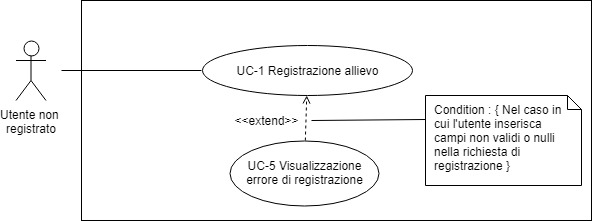
\includegraphics[scale=0.7]{images/UC-1_a.png}
	\caption{UC-1 Registrazione Allievo}
\end{figure}

\subsubsection{UC-33 Registrazione Insegnante}
\begin{itemize}
	\item \textbf{Attori: }Utente non registrato.
	\item \textbf{Precondizione: }L'utente si trova nella vista di registrazione dell'applicazione.
	\item \textbf{Postcondizione: }L'utente è in attesa di conferma.
	\item \textbf{Scenario principale: }
	\begin{enumerate}
		\item l'utente ha scelto di registrarsi al sistema, quindi di creare un nuovo profilo
		\item l'utente seleziona la tipologia insegnante
		\item l'utente inserirà nome, cognome, username, email e password
		\item l'utente fornirà il nome della scuola a cui appartiene e la città
		\item l'utente inserirà il proprio codice INPS
		\item l'utente conferma la registrazione
	\end{enumerate}
	\item \textbf{Estensioni: }
	\begin{itemize}
		\item 5.a Nel caso in cui l'utente tenti l'inserimento di campi non validi vedrà comparire dei messaggi d'errore "Campi non validi" (UC-5).
	\end{itemize}
\end{itemize}

\begin{figure}[h]
	\centering
	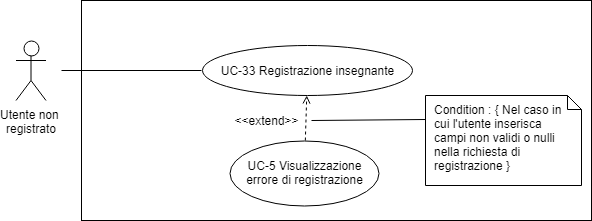
\includegraphics[scale=0.7]{images/UC-1i.png}
	\caption{UC-33 Registrazione Insegnante}
\end{figure}	

\subsubsection{UC-5 Visualizzazione errore di registrazione}
\begin{itemize}
	\item \textbf{Attori:} Utente non registrato
	\item \textbf{Precondizione:} L'utente ha confermato la richiesta di registrazione con campi non validi o nulli
	\item \textbf{Postcondizione:} L'utente torna alla vista di registrazione
	\item  \textbf{Scenario principale: }
	\begin{enumerate}
		\item visualizza un messaggio di errore "Registrazione non avvenuta: campi non validi"
	\end{enumerate}
\end{itemize}

\subsubsection{UC-36 Notifica richiesta insegnante}
   \begin{itemize}
   \item \textbf{Attori:} Utente non registrato
   \item \textbf{Precondizione:} L'utente ha inviato la richiesta di registrazione come insegnante.
   \item \textbf{Postcondizione:} L'utente riceve la conferma di registrazione come insegnante. 
   \item \textbf{Scenario principale:}
    \begin{enumerate}
     \item l'utente riceve una notifica della conferma via e-mail
    \end{enumerate}
  \end{itemize}


\subsection{Elenco dei casi d'uso - Utente: Utente non autenticato}
\subsubsection{UC-2 Autenticazione}
		\begin{itemize}
			\item \textbf{Attori:} Utente non autenticato.
			\item \textbf{Precondizione:} L'utente si trova nella vista di autenticazione dell'applicazione.
			\item \textbf{Postcondizione:} L'utente ha eseguito l'accesso con il proprio ruolo.
			\item \textbf{Scenario principale:}
				\begin{enumerate}
					\item l'utente inserisce propri username e password
					\item l'utente conferma l'accesso
				\end{enumerate}
				\item \textbf{Estensioni:}
				\begin{itemize}
					\item 2.a Nel caso in cui l'utente tenti l'inserimento di campi non validi vedrà comparire un messaggio d'errore (UC-34).
				\end{itemize}
		\end{itemize}
		
\subsubsection{UC-34 Visualizzazione errore di autenticazione}
		\begin{itemize}
			\item \textbf{Attori:} Utente non autenticato
			\item \textbf{Precondizione:} L'utente ha provato ad autenticarsi.
			\item \textbf{Postcondizione:} L'utente torna alla vista di accesso alla piattaforma.
			\item \textbf{Scenario principale:}
			\begin{enumerate}
				\item l'utente visualizza un messaggio di errore "Impossibile effettuare l'accesso: username o password errati"
			\end{enumerate}
		\end{itemize}
		
\subsection{Elenco dei casi d'uso - Utente: utente registrato}
\subsubsection{UC-55 Visualizzazione profilo personale}
\begin{itemize}
	\item \textbf{Attori:} Utente registrato
	\item \textbf{Precondizione:} L'utente si trova nella vista principale dell'applicazione.
	\item \textbf{Postcondizione:} L'utente si trova nella vista del proprio profilo.
	\item \textbf{Scenario principale:}
		\begin{enumerate}
			\item l'utente seleziona la voce "Profilo personale"
		\end{enumerate}
\end{itemize}

\subsubsection{UC-3 Modifica profilo}
		\begin{itemize}
			\item \textbf{Attori:} Utente registrato.
			\item \textbf{Precondizione:} L'utente si trova nella vista di modifica dei dati del proprio profilo.
			\item \textbf{Postcondizione:} L'utente ha modificato i propri dati personali.
			\item \textbf{Scenario principale:}
				\begin{enumerate}
					\item l'utente modifica username, password, scuola o città
					\item L'utente conferma la modifica
				\end{enumerate}
				\item \textbf{Estensioni:}
				\begin{itemize}
					\item 2.a Nel caso in cui l'utente tenti l'inserimento di campi non validi vedrà comparire un messaggio d'errore (UC-35).
				\end{itemize}
		\end{itemize}
		\begin{figure}[htbp]
			\centering
			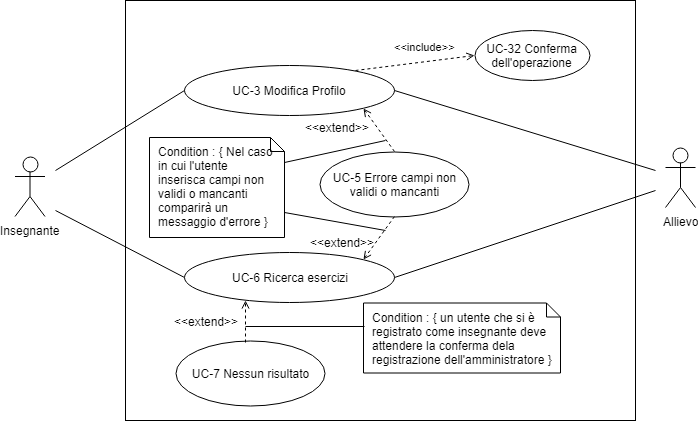
\includegraphics[scale=0.7]{images/UC-3.png}
			\caption{UC-3 Modifica profilo}
		\end{figure}
	
\subsubsection{UC-35 Visualizzazione errore di modifica del profilo}	
	\begin{itemize}
		\item \textbf{Attori:} Utente registrato
		\item \textbf{Precondizione:} L'utente ha inserito dei campi non validi o nulli nella modifica del proprio profilo.
		\item \textbf{Postcondizione:} L'utente torna alla vista del proprio profilo.
		\item \textbf{Scenario principale:}
		\begin{enumerate}
			\item l'utente visualizza un messaggio di errore "Modifica del profilo non avvenuta: campi non validi o nulli"
		\end{enumerate}
	\end{itemize}

\subsection{Elenco dei casi d'uso - Utente: moderatore}	
\subsubsection{UC-4 Verifica richiesta insegnante}
		\begin{itemize}
			\item \textbf{Attori:} Moderatore.
			\item \textbf{Precondizione:} Il moderatore si trova nella vista di amministrazione dell'applicazione.
			\item \textbf{Postcondizione:} Il moderatore ha confermato o rifiutato l'utente richiedente il ruolo di insegnante.
			\item \textbf{Scenario principale:}
				\begin{enumerate}
					\item il moderatore visualizza la lista degli utenti che richiedono il ruolo di insegnante
					\item il moderatore accetta o rifiuta l'utente selezionato
				\end{enumerate}
		\end{itemize}		
			
\subsubsection{UC-50 Visualizzazione lista degli esercizi: moderatore}
	\begin{itemize}
		\item \textbf{Attori:} Moderatore.
		\item \textbf{Precondizione:} Il moderatore si trova nella vista di amministrazione dell'applicazione.
		\item \textbf{Postcondizione:} Il moderatore visualizza la lista degli esercizi inseriti nella piattaforma.
		\item \textbf{Scenario principale:}
			\begin{enumerate}
				\item il moderatore seleziona l'opzione "Esercizi"
			\end{enumerate}
	\end{itemize}
		
\subsubsection{UC-51 Ricerca esercizi: moderatore}
	\begin{itemize}
		\item \textbf{Attori:} Moderatore.
		\item \textbf{Precondizione:} Il moderatore visualizza la lista degli esercizi inseriti nella piattaforma.
		\item \textbf{Postcondizione:} Il moderatore ottiene una lista degli esercizi contenenti la parola o le parole cercate.
		\item \textbf{Scenario principale:}
			\begin{enumerate}
				\item il moderatore scrive nella barra di ricerca una frase o una sua parte
			\end{enumerate}
	\end{itemize}
	
\subsubsection{UC-23 Eliminazione di un esercizio}
			\begin{itemize}
			\item \textbf{Attori:} Moderatore.
			\item \textbf{Precondizione:} Il moderatore visualizza la lista di esercizi.
			\item \textbf{Postcondizione:} Il moderatore ha eliminato l'esercizio desiderato.
			\item \textbf{Scenario principale:}
				\begin{enumerate}
					\item il moderatore indica gli esercizi da eliminare
					\item il moderatore conferma l'eliminazione dell'esercizio selezionato
				\end{enumerate}
		\end{itemize}

\subsubsection{UC-52 Visualizzazione lista degli utenti: moderatore}
	\begin{itemize}
		\item \textbf{Attori:} Moderatore.
		\item \textbf{Precondizione:} Il moderatore si trova nella vista di amministrazione dell'applicazione.
		\item \textbf{Postcondizione:} Il moderatore visualizza la lista degli utenti presenti nella piattaforma.
		\item \textbf{Scenario principale:}
			\begin{enumerate}
				\item il moderatore seleziona l'opzione "Utenti"
			\end{enumerate}
	\end{itemize}
		
\subsubsection{UC-53 Ricerca utenti: moderatore}
	\begin{itemize}
		\item \textbf{Attori:} Moderatore.
		\item \textbf{Precondizione:} Il moderatore visualizza la lista degli utenti presenti nella piattaforma.
		\item \textbf{Postcondizione:} Il moderatore ottiene una lista degli utenti aventi nell'username la parola indicata.
		\item \textbf{Scenario principale:}
			\begin{enumerate}
				\item il moderatore scrive nella barra di ricerca una stringa
			\end{enumerate}
	\end{itemize}

\subsubsection{UC-8 Eliminazione di un utente}
\begin{itemize}
	\item \textbf{Attori:} Moderatore.
	\item \textbf{Precondizione:} Il moderatore visualizza la lista degli utenti.
	\item \textbf{Postcondizione:} Il moderatore ha eliminato l'utente desiderato.
	\item \textbf{Scenario principale:}
	\begin{enumerate}
		\item il moderatore indica uno o più utenti da eliminare
		\item il moderatore conferma l'eliminazione degli utenti selezionati
	\end{enumerate}
\end{itemize}

\subsubsection{UC-47 Visualizzazione lista delle segnalazioni}
\begin{itemize}
	\item \textbf{Attori:} Moderatore.
	\item \textbf{Precondizione:} Il moderatore si trova nella vista di amministrazione dell'applicazione.
	\item \textbf{Postcondizione:} Il moderatore visualizza la lista delle segnalazioni ricevute.
	\item \textbf{Scenario principale:}
	\begin{enumerate}
		\item Il moderatore seleziona l'opzione "Lista delle segnalazioni"
	\end{enumerate}
\end{itemize}

\subsubsection{UC-48 Eliminazione segnalazione}
\begin{itemize}
	\item \textbf{Attori:} Moderatore.
	\item \textbf{Precondizione:} Il moderatore visualizza la lista delle segnalazioni ricevute.
	\item \textbf{Postcondizione:} Il moderatore ha eliminato la segnalazione desiderata.
	\item \textbf{Scenario principale:}
	\begin{enumerate}
		\item Il moderatore seleziona la segnalazione
		\item Il moderatore seleziona l'opzione "Elimina segnalazione"
	\end{enumerate}
\end{itemize}

\subsection{Elenco dei casi d'uso - Utente: insegnante}		
\subsubsection{UC-10 Visualizzazione esercizi inseriti}
\begin{itemize}
\item \textbf{Attori: }Insegnante.
		\item \textbf{Precondizione: }L'insegnante si trova nell'area del suo profilo.
		\item \textbf{Postcondizione: }L'insegnante visualizza una lista di esercizi inseriti. 
		\item \textbf{Scenario principale:}
		\begin{enumerate}
			\item l'insegnante seleziona la voce "Esercizi inseriti"
		\end{enumerate}
	\end{itemize}

\subsubsection{UC-54 Ricerca esercizi inseriti}
\begin{itemize}
	\item \textbf{Attori:} Insegnante.
	\item \textbf{Precondizione:} L'insegnante visualizza la lista degli esercizi che ha inserito nella piattaforma.
	\item \textbf{Postcondizione:} L'insegnante ottiene la lista degli esercizi contenenti la parola o le parole cercate.
	\item \textbf{Scenario principale:}
		\begin{enumerate}
				\item l'insegnante scrive nella barra di ricerca una frase o una sua parte
		\end{enumerate}
\end{itemize}

\subsubsection{UC-9 Modifica soluzione}
\begin{itemize}
	\item \textbf{Attori:} Insegnante.
	\item \textbf{Precondizione:} L'insegnante ha selezionato dalla lista degli esercizi inseriti.
	\item \textbf{Postcondizione:} La soluzione inserita è stata modificata.
	\item \textbf{Scenario principale:}
		\begin{enumerate}
		\item l'insegnante visualizza le parole della frase associate alle classi grammaticali indicati nella precedente soluzione
		\item l'insegnante modifica le classi grammaticali associate alle parole dell'esercizio
		\item l'insegnante conferma la modifica
		\end{enumerate}
\end{itemize}
	
\subsubsection{UC-11 Eliminare una soluzione di un esercizio}
\begin{itemize}
	\item \textbf{Attori:} Insegnante.
	\item \textbf{Precondizione:} L'insegnante visualizza la lista degli esercizi inseriti.
	\item \textbf{Postcondizione:} Le soluzioni selezionate vengono eliminate.
	\item \textbf{Scenario principale:}
		\begin{enumerate}
			\item l'insegnante seleziona una o più soluzioni da eliminare
			\item l'insegnante conferma l'eliminazione
		\end{enumerate}
\end{itemize}

\subsubsection{UC-12 Inserimento esercizio}
	\begin{itemize}
		\item \textbf{Attori: }Insegnante.
		\item \textbf{Precondizione: }L'insegnante è nella vista di inserimento di un nuovo esercizio.
		\item \textbf{Postcondizione: }L'esercizio è stato inserito.
		\item \textbf{Scenario principale: }
			\begin{enumerate} 
				\item l'insegnante inserisce la frase
				\item l'insegnante inserisce la soluzione UC-12.1
				\item l'insegnante inserisce gli argomenti UC-12.2
				\item l'insegnante inserisce la difficoltà UC-12.3
				\item l'insegnante conferma l'inserimento
			\end{enumerate}
		\item \textbf{Estensioni:} 
			\begin{itemize}
				\item 1.a Nel caso in cui la frase inserita sia nulla, viene visualizzato un errore (UC-37)
			\end{itemize}
	\end{itemize}
	\begin{figure}[h]
		\centering
		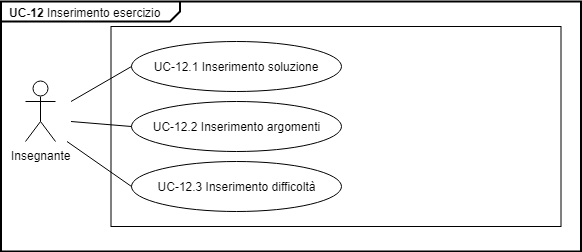
\includegraphics[scale=0.7]{images/UC-12.png}
		\caption{UC-12 Inserimento esercizio}
	\end{figure}

\subsubsection{UC-12.1 Inserimento di una soluzione}
\begin{itemize}
\item \textbf{Attori: }Insegnante.
\item \textbf{Precondizione: }L'insegnante è nella vista di inserimento di un nuovo esercizio.
\item \textbf{Postcondizione: }L'insegnante ha inserito la propria soluzione.
\item \textbf{Scenario principale: }
		\begin{enumerate} 
		\item l'insegnante visualizza la soluzione proposta dal generatore automatico
		\item l'insegnante può modificare le classi grammaticali assegnate dal generatore automatico che ritiene errate
		\item l'insegnante seleziona lo stato della soluzione inserita, pubblica o privata
		\item l'insegnante conferma la soluzione
		\end{enumerate}	
\end{itemize}

\subsubsection{UC-12.2 Inserimento argomenti}
\begin{itemize}
\item \textbf{Attori: }Insegnante.

\item \textbf{Precondizione:} L'insegnante sta inserendo un esercizio, gli viene richiesta la compilazione di una lista di argomenti presenti nell'esercizio.
\item \textbf{Postcondizione:} L'insegnante ha selezionato gli argomenti trattati nell'esercizio.
\item \textbf{Scenario principale: }
		\begin{enumerate}
		\item l'insegnante visualizza la lista degli argomenti
		\item l'insegnante seleziona gli argomenti che vengono toccati nell'esercizio
		\end{enumerate}
\end{itemize}				

\subsubsection{UC-12.3 Inserimento della difficoltà}
\begin{itemize}
	\item \textbf{Attori: }Insegnante
	\item \textbf{Precondizione:} L'insegnante è nella vista di inserimento di un nuovo esercizio.
	\item \textbf{Postcondizione:} L'insegnante ha indicato il livello di difficoltà.
	\item \textbf{Scenario principale:}
	\begin{enumerate}
		\item l'insegnante visualizza i livelli possibili di difficoltà (da 1 a 5)
		\item l'insegnante indica il livello di difficoltà dell'esercizio da inserire
	\end{enumerate}
\end{itemize}

\subsubsection{UC-37 Visualizzazione errore di inserimento di una frase vuota}
\begin{itemize}
	\item \textbf{Attori:} Insegnante
	\item \textbf{Precondizione:} L'insegnante è nella vista di inserimento di un nuovo esercizio e ha inserito una frase vuota.
	\item \textbf{Postcondizione:} L'insegnante torna alla vista di inserimento dell'esercizio.
	\item \textbf{Scenario principale:}
	\begin{enumerate}
		\item l'insegnante visualizza un messaggio di errore "La frase inserita è vuota"
	\end{enumerate}
\end{itemize}

\subsubsection{UC-24 Creazione di una classe}
\begin{itemize}
	\item \textbf{Attori:} Insegnante.
	\item \textbf{Precondizione:} L'insegnante si trova nella vista del proprio profilo.
	\item \textbf{Postcondizione:} L'insegnante si trova nella vista di gestione della classe creata.
	\item \textbf{Scenario principale:}
	\begin{enumerate}
		\item l'insegnante selezione l'opzione "Crea classe"
		\item l'insegnante assegna un nome alla classe
		\item l'insegnante assegna una descrizione alla classe
		\item l'insegnante conferma la creazione
	\end{enumerate}
\end{itemize}

\subsubsection{UC-25 Eliminazione di una classe}
\begin{itemize}
	\item \textbf{Attori:} Insegnante.
	\item \textbf{Precondizione:} L'insegnante si trova nella vista di gestione di una propria classe.
	\item \textbf{Postcondizione:} L'insegnante elimina la classe dal sistema.
	\item \textbf{Scenario principale:}
	\begin{enumerate}
		\item l'insegnante clicca sul pulsante di eliminazione della classe
		\item l'insegnante conferma l'eliminazione
	\end{enumerate}
\end{itemize}

\subsubsection{UC-26 Inserimento alunni}
\begin{itemize}
	\item \textbf{Attori:} Insegnante.
	\item \textbf{Precondizione:} L'insegnante si trova nella vista di gestione di una propria classe.
	\item \textbf{Postcondizione:} L'insegnante visualizza gli alunni inseriti.
	\item \textbf{Scenario principale:}
	\begin{enumerate}
		\item l'insegnante seleziona l'opzione "Aggiungi alunni"
		\item l'insegnante indica gli studenti da aggiungere (UC-26.1)
		\item l'insegnante conferma l'inserimento
	\end{enumerate}
\end{itemize}

\subsubsection{UC-26.1 Selezione alunni per l'inserimento}
\begin{itemize}
	\item \textbf{Attori:} Insegnante
	\item \textbf{Precondizione:} l'insegnante si trova nella vista di aggiunta degli alunni a una classe
	\item \textbf{Postcondizione:} l'insegnante ha indicato gli alunni da inserire nella classe
	\item \textbf{Scenario principale:}
	\begin{enumerate}
		\item l'insegnante visualizza la lista di tutti gli alunni presenti sulla piattaforma
		\item l'insegnante ricerca gli alunni da inserire (UC-26.1.1)	
		\item l'insegnante seleziona gli alunni da inserire
	\end{enumerate}
\end{itemize}

\subsubsection{UC-26.1.1 Ricerca alunno}
\begin{itemize}
	\item \textbf{Attori:} Insegnante
	\item \textbf{Precondizione:} l'insegnante visualizza la lista di tutti gli alunni presenti sulla piattaforma.
	\item \textbf{Postcondizione:} l'insegnante visualizza una lista di username contenenti la stringa inserita.
	\item \textbf{Scenario principale:}
	\begin{enumerate}
		\item l'insegnante scrive l'username di un alunno, o una sua parte
	\end{enumerate}
\end{itemize}

\subsubsection{UC-27 Assegnazione esercizi}
\begin{itemize}
	\item \textbf{Attori:} Insegnante.
	\item \textbf{Precondizione:} Visualizza una lista di esercizi da una ricerca eseguita.
	\item \textbf{Postcondizione:} L'insegnante ha assegnato esercizi alla classe.
	\item \textbf{Scenario principale:}
	\begin{enumerate}
		\item l'insegnante seleziona degli esercizi in lista da assegnare
		\item l'insegnante indica la classe a cui assegnarli
		\item l'insegnante conferma l'assegnazione
	\end{enumerate}
\end{itemize}

\subsubsection{UC-31 Visualizza lista delle classi}		
\begin{itemize}
	\item \textbf{Attori:} Insegnante.
	\item \textbf{Precondizione:} L'insegnante si trova nella vista del proprio profilo.
	\item \textbf{Postcondizione:} L'insegnante visualizza la lista delle classi create.
	\item \textbf{Scenario principale:}
	\begin{enumerate}
		\item l'insegnante seleziona l'opzione "vedi classi"
	\end{enumerate}		
\end{itemize}

\subsubsection{UC-49 Visualizzazione area di gestione di una classe}
\begin{itemize}
	\item \textbf{Attori:} Insegnante.
	\item \textbf{Precondizione:} L'insegnante visualizza la lista delle classi create.
	\item \textbf{Postcondizione:} L'insegnante visualizza la vista di gestione di una propria classe.
	\item \textbf{Scenario principale:}
	\begin{enumerate}
		\item l'insegnante seleziona una classe
	\end{enumerate}
\end{itemize}

\subsubsection{UC-30 Visualizza lista degli alunni iscritti alla classe}		
\begin{itemize}
	\item \textbf{Attori:} Insegnante.
	\item \textbf{Precondizione:} L'insegnante si trova nella vista di gestione di una propria classe.
	\item \textbf{Postcondizione:} L'insegnante visualizza l'elenco degli alunni iscritti.
	\item \textbf{Scenario principale:}
	\begin{enumerate}
		\item l'insegnante seleziona l'opzione "vedi alunni"
	\end{enumerate}		
\end{itemize}

\subsubsection{UC-28 Visualizzare i progressi di un alunno della classe}
\begin{itemize}
	\item \textbf{Attori:} Insegnante.
	\item \textbf{Precondizione}: L'insegnante visualizza l'elenco degli alunni iscritti alla classe.
	\item \textbf{Postcondizione:} L'insegnante visualizza i progressi relativi allo studente selezionato.
	\item \textbf{Scenario principale:}
	\begin{enumerate}
		\item l'insegnante seleziona uno studente
		\item l'insegnante visualizza i grafici che riportano la media totale, la media per tipologia di esercizi e lo sviluppo della media nel tempo
	\end{enumerate}
\end{itemize}

\subsubsection{UC-29 Elimina alunno dalla classe}		
\begin{itemize}
	\item \textbf{Attori:} Insegnante.
	\item \textbf{Precondizione:} L'insegnante visualizza la lista degli alunni della classe.
	\item \textbf{Postcondizione:} L'insegnante ha rimosso l'allievo dalla classe.
	\item \textbf{Scenario principale:}
	\begin{enumerate}
		\item l'insegnante seleziona l'allievo da rimuovere dalla classe
		\item l'insegnante conferma l'eliminazione
	\end{enumerate}	
\end{itemize}


\subsection{Elenco dei casi d'uso - Utente: allievo}
	\subsubsection{UC-14 Visualizzazione progressi}
	\begin{itemize}
			\item \textbf{Attori:} Allievo.
			\item \textbf{Precondizione:} L'allievo si trova nella vista del proprio profilo.
			\item \textbf{Postcondizione:} L'allievo visualizza i progressi svolti fino a quel momento.
			\item \textbf{Scenario principale:}
				\begin{enumerate}
					\item L'allievo visualizza la media delle valutazioni ricevute, la media per tipologia di esercizi e lo sviluppo della media nel tempo
				\end{enumerate}
	\end{itemize}
	
	\subsubsection{UC-7 Visualizzazione lista delle classi di appartenenza}
		\begin{itemize}
			\item \textbf{Attori:} Allievo.
			\item \textbf{Precondizione:} L'allievo si trova nella vista del proprio profilo.
			\item \textbf{Postcondizione:} L'allievo visualizza la lista delle classi a cui appartiene.
			\item \textbf{Scenario principale:}
			\begin{enumerate}
				\item L'allievo seleziona l'opzione "Lista delle classi"
			\end{enumerate}
		\end{itemize}			

	\subsubsection{UC-32 Annullamento dell'iscrizione a una classe}
		\begin{itemize}
			\item \textbf{Attori:} Allievo.
			\item \textbf{Precondizione:} L'allievo visualizza la lista delle classi a cui appartiene.
			\item \textbf{Postcondizione:} L'allievo ha annullato l'iscrizione alla classe.
			\item \textbf{Scenario principale:}
			\begin{enumerate}
				\item l'allievo seleziona l'opzione "Disiscriviti" in corrispondenza di una classe
			\end{enumerate}
		\end{itemize}					
				
	\subsubsection{UC-45 Visualizzazione delle informazioni della classe}
		\begin{itemize}
			\item \textbf{Attori:} Allievo.
			\item \textbf{Precondizione:} L'allievo visualizza la lista delle classi a cui appartiene.
			\item \textbf{Postcondizione:} L'allievo visualizza le informazioni della classe indicata (allievi iscritti e media delle valutazioni).
			\item \textbf{Scenario principale:}
			\begin{enumerate}
				\item l'allievo seleziona una classe
			\end{enumerate}
		\end{itemize}